
% JuliaCon proceedings template
\documentclass{juliacon}
\setcounter{page}{1}

\begin{document}

% **************GENERATED FILE, DO NOT EDIT**************

\title{BlankLocalizationCore.jl: implementing blank localization in Julia}

\author[1, 2]{Tamás Cserteg}
\author[1]{András Kovács}
\author[1, 3]{József Váncza}
\affil[1]{EPIC Centre of Excellence, HUN-REN Institute for Computer Science and Control (SZTAKI), Budapest H-1111, Hungary}
\affil[2]{Doctoral School of Informatics, ELTE Eötvös Loránd University, Budapest H-1117, Hungary}
\affil[3]{Department of Manufacturing Science and Technology, Budapest University of Technology and Economics, Budapest H-1111, Hungary}

\keywords{Julia, Optimization, Machining, Blank localization}

\hypersetup{
pdftitle = {BlankLocalizationCore.jl: implementing blank localization in Julia},
pdfsubject = {JuliaCon 2022 Proceedings},
pdfauthor = {Tamás Cserteg, András Kovács, József Váncza},
pdfkeywords = {Julia, Optimization, Machining, Blank localization},
}



\maketitle

\begin{abstract}

Blank localization (also known as workpiece referencing) is an essential task in machining.
It aims to precisely establish the geometric relation of the machine tool (mill, lathe, etc.) and the workpiece.
We introduced the concept of multi-operation blank localization to address this task for drilling and milling scenarios in a semi-automated way,
which allows positioning different machining features (e.g., different holes) separately in order to exploit the tolerances on the relative position of those features to compensate the small errors of the blank.
The method takes as input the measured rough geometry and the machining CNC code, and computes the best possible position of each feature considering machining allowances and tolerances by solving a convex quadratically constrained quadratic program (QCQP).
The versatility and extensibility of the Julia language helped the development of this algorithm, materializing in the \texttt{BlankLocalizationCore.jl} package.
Its flexibility and ease of use make it an excellent research tool that can be deployed in production as well.
\end{abstract}

\section{Introduction}
\label{sec:intro}
Cast parts may have small geometric variations from lot to lot that need to be addressed before machining by altering the CNC code.
Current practice is dominated by iterative adjustments by human operators, which requires highly trained workers and takes a long time.
Automated methods exist for complex free-form parts like wind turbines that place the entire blank as a single solid object \cite{tan:2014_UnconstrainedApproachBlank}.
Multi-operation blank localization~\cite{cserteg:2023_Annals} however handles groups of features independently, providing greater flexibility than traditional approaches.
It focuses on drilling and milling which are among the most common machining operations, making it applicable to a wide range of products.
The abstract method and its implementation were developed in parallel, which required a language with wide variety of tools and support for easy prototyping.
Exactly for these reasons we chose the Julia language~\cite{bezanson2017julia}.

\section{Multi-operation blank localization}
\label{sec:algo}

The problem involves looking for the optimal position for each to-be-machined feature (short: machined feature) on the workpiece.
These features are grouped together, with each group defined relative to a specific reference point known as the part zero.
The layout of these part zeros is controlled by the structure of the machining CNC code.
By moving the part zeros, we can indirectly control the positions of the associated features.
Each part zero—and by extension, each group—can be moved independently, which gives the method its flexibility.
In the optimization program, the positions of the part zeros are the decision variables.

To ensure the required surface finish, the machined features must enclose the pre-cast features on the blank (called rough features) with a minimum machining allowance (a lower bound parameter).
The allowance calculation requires the final part specification in the form of the machining CNC code as well as a representation of the rough geometries.
From their positions and geometric parameters their distance can be computed, which then can be used to generate the allowance constraints for the optimization program.

The other set of constraints roots from respecting the dimensional tolerances describing functional properties (e.g. connections to mating parts).
The developed tolerance model encodes the distance of machined-machined (or sometimes machined-rough) features as axis-aligned minimum and maximum distance.
Fig.~\ref{fig:hatfig} from \cite{cserteg:2023_Annals} shows some examples for these features.

\begin{figure}[b]
	\centerline{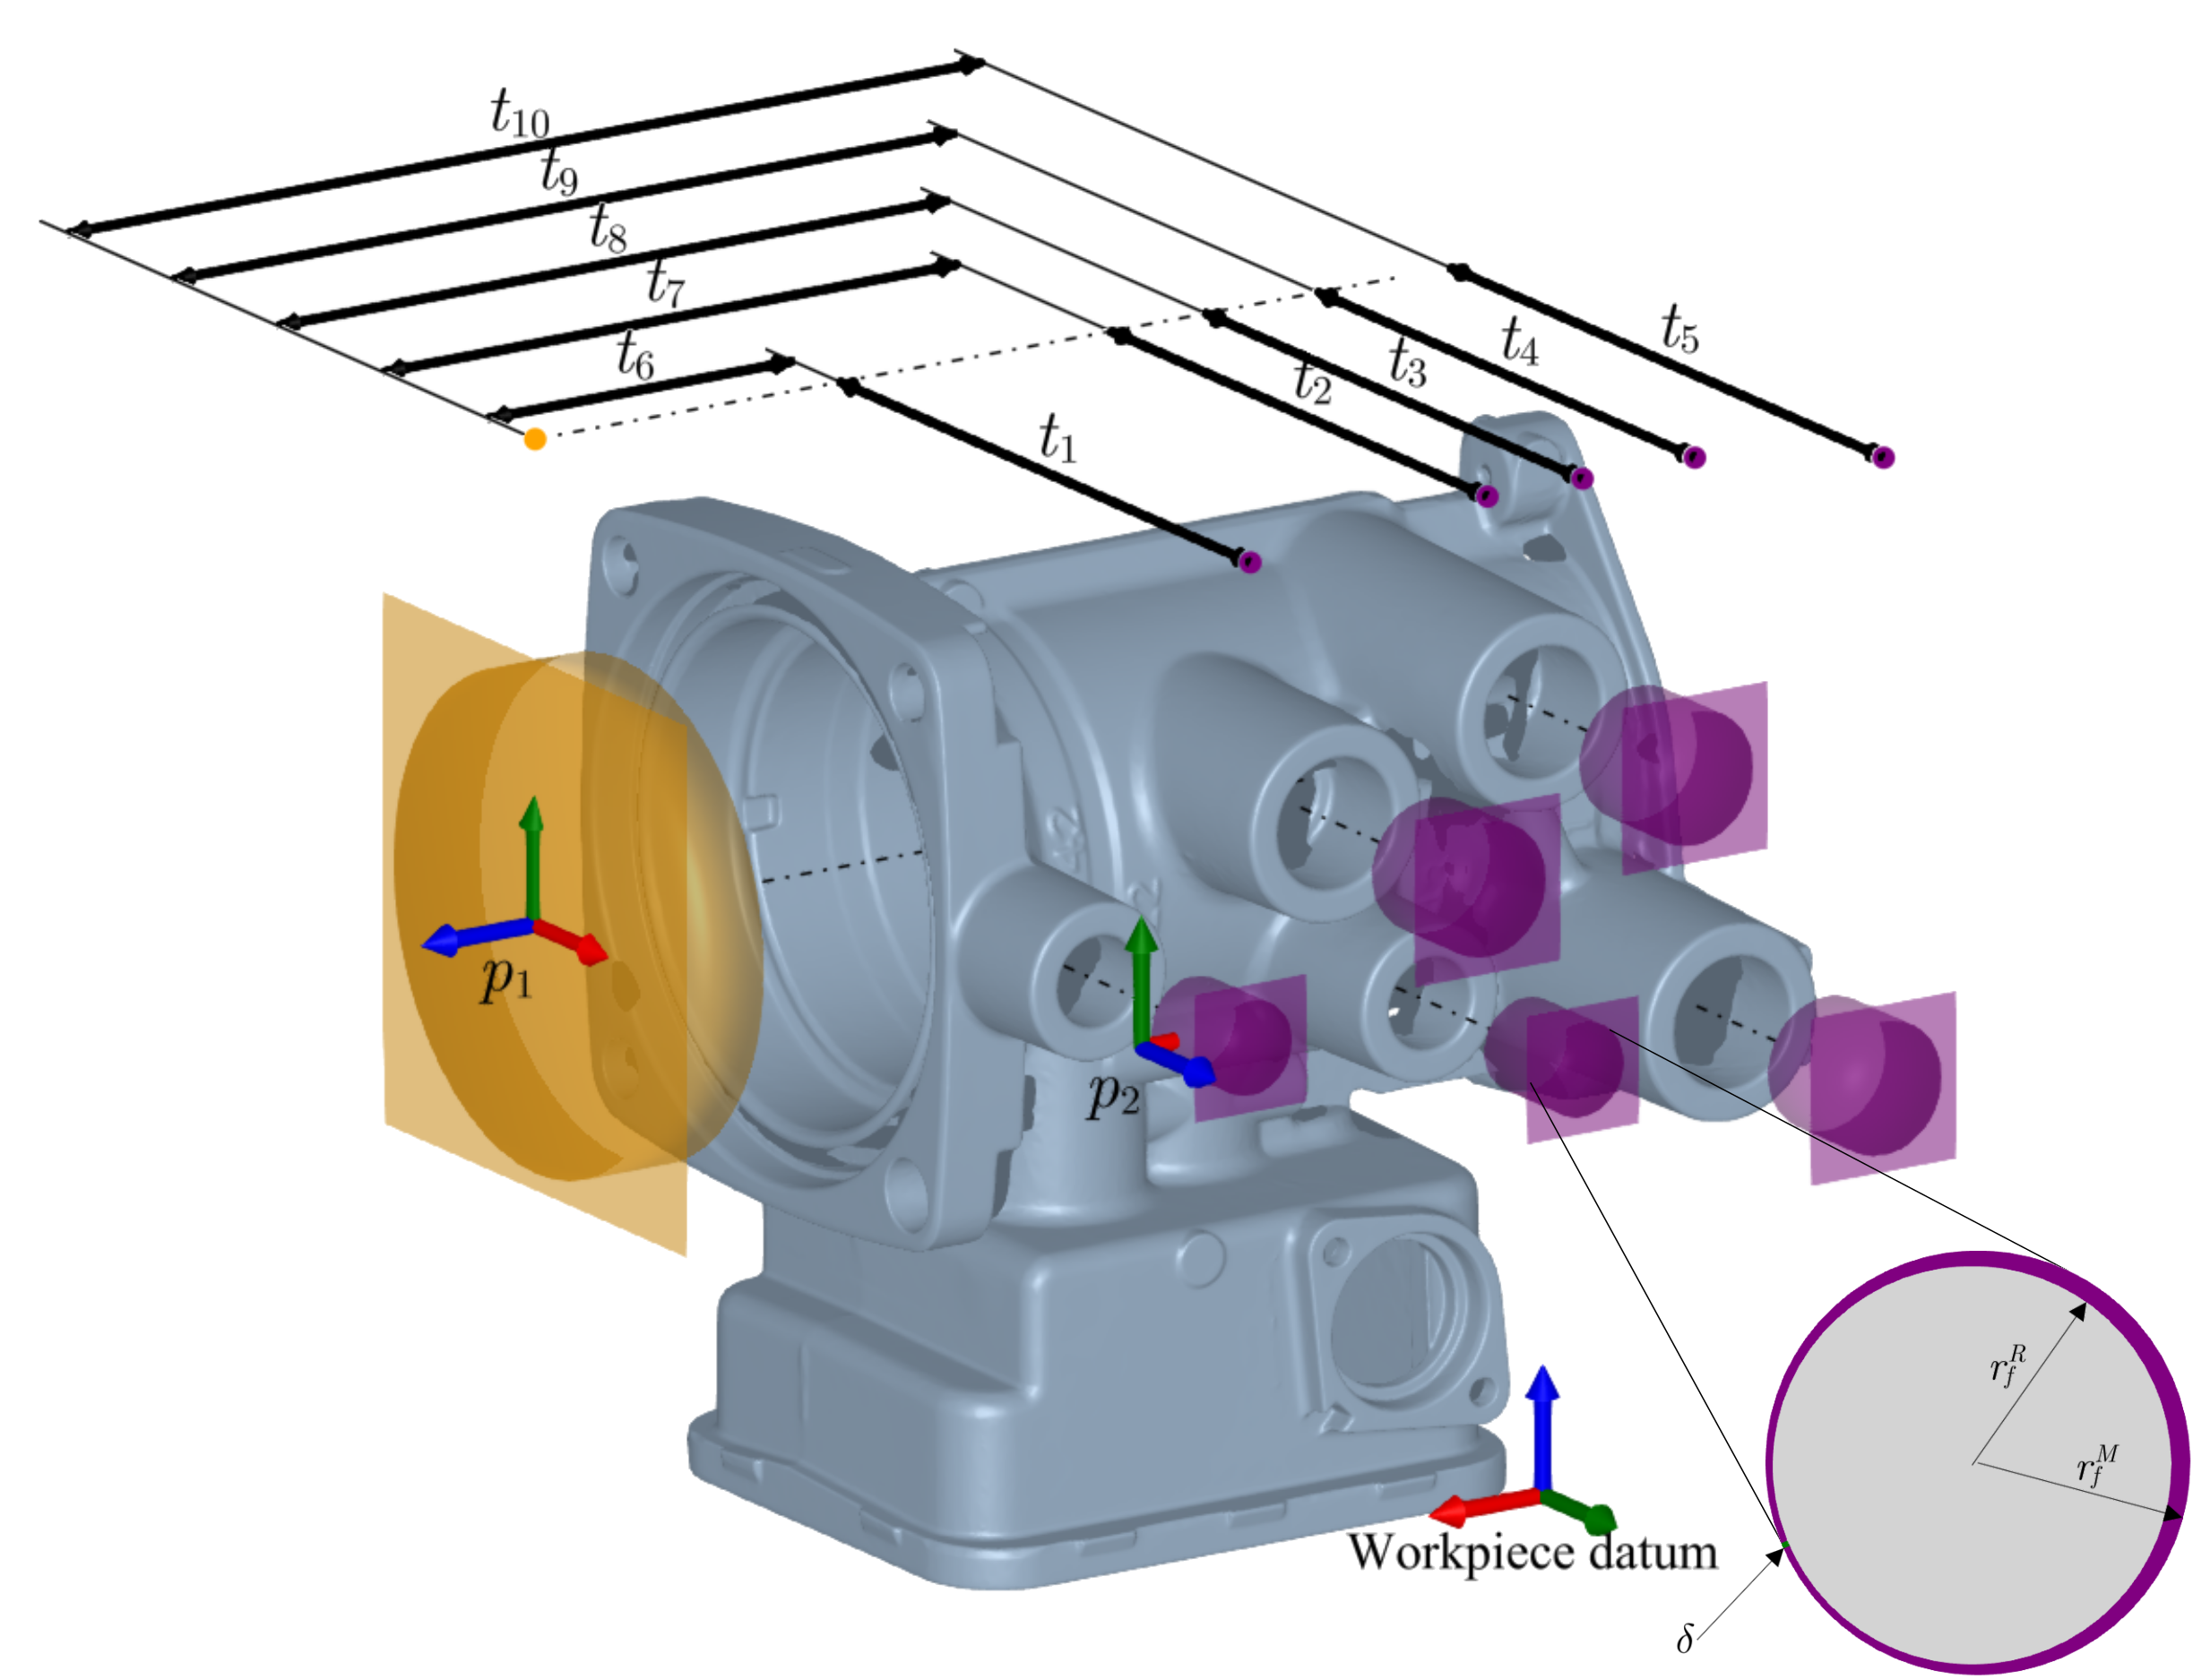
\includegraphics[width=0.95\columnwidth]{cirp-annals-2023-figure-2.png}}
	\caption{3D scanned rough features (in grey), two machined feature groups (orange and purple) with their part zeros, and tolerances connecting the machined features~\cite{cserteg:2023_Annals}.}
	\label{fig:hatfig}
\end{figure}

Following common machining practice, the objective of the optimization program is to achieve as little tolerance deviation as possible.
The problem is formulated as a convex quadratically constrained quadratic program (convex QCQP).
The optimization model itself and use-cases are described in \cite{cserteg:2023_CMS} and \cite{cserteg:2023_Annals}, while implementation details are given in the following section.

\section{Implementation in Julia}
\label{sec:approach}

Julia enabled us to develop an implementation with the following properties:
\begin{itemize}
	\item Concise interface to generate the parameters of the declarative optimization program based on procedural geometric calculations.
	\item Support for a variety of geometrical representations, especially regarding the differences of drilling/milling operations and free-form/primitive geometry representations.
	\item Support for analyzing and visualizing the results.
\end{itemize}

The implementation is built around JuMP~\cite{Lubin2023}, which serves as the interface to the underlying optimization solver.
With JuMP's excellent design, combining the necessary geometric calculations and the declarative optimization program definition was straightforward.
Other advantage of JuMP is that solvers can be easily swapped.
For development, the (commercial) FICO Xpress solver was used, but our industry partner could use the (open source) Ipopt or SCIP solvers without issue.

To handle the tolerance and allowance calculations, the part definition (CNC code), rough geometry measurements and tolerances need to be stored.
Their representation is built upon a flexible geometry type system.

The CNC code can be represented with plane and cylinder geometries for milling and drilling operations.
This "type" information of the geometries is encoded with Julia types.
The primitive or free-form nature of the geometries is implemented with the holy traits pattern and is necessary because different instruments output different types of geometric data.
For example, a coordinate measurement machine will provide primitive geometry definitions like disks and cylinders, while a 3D scanner outputs point clouds or meshes (called free-form collectively).
The \texttt{IsPrimitve} or \texttt{IsFreeForm} traits are applied to geometry types independently of their planar or cylindrical type.
Code block~\ref{lst:def-types} shows a shortened version of the implemented type system.

\begin{lstlisting}[language = Julia, numbers=left, label={lst:def-types}, caption={Shortened implementation of the type system used by \texttt{BlankLocalizationCore.jl}.}]
# Type tree for localization geometries.
# "ALoc": AbstractLocalization
abstract type ALocGeometry end
abstract type AHoleGeometry <: ALocGeometry end
abstract type APlaneGeometry <: ALocGeometry end

# Trait to describe the "style" of an ALocGeometry.
abstract type GeometryStyle end
struct IsPrimitive <: GeometryStyle end
struct IsFreeForm <: GeometryStyle end
\end{lstlisting}

The optimization model uses a "feature point" concept which requires the position and some parameters of the geometries.
A function interface is designed for accessing these values.
The package documentation contains the list of functions that need to be defined but some are showcased in code block~\ref{lst:example}.
One function that we want to highlight is the \texttt{visualizationgeometry}, which needs to return a \texttt{Meshes.jl} object that will be passed to the \texttt{Meshes.viz} function.
Using the Meshes ecosystem~\cite{Hoffimann2023}, we could not only interactively inspect the results of the optimization, but also produce publication quality images, like Fig.~\ref{fig:hatfig}.

\vspace*{1em}

\begin{lstlisting}[language = Julia, numbers=left, label={lst:example}, caption={Defining a new type for the optimization model.}]
struct MyDisk <: AHoleGeometry
  p::Vector{Float64} # center point
  n::Vector{Float64} # surface normal
  d::Float64 # diameter
end

GeometryStyle(::Type{MyDisk}) = IsPrimitive()

featurepoint(::IsPrimitive, x::MyDisk) = x.p
featureradius(::IsPrimitive, x::MyDisk) = x.d/2

using Meshes

function visualizationgeometry(geom::MyDisk)
  plane = Plane(Point3(geom.p), Vec3(geom.n))
  return Disk(plane, geom.d/2)
end
\end{lstlisting}

\section{Results and future work}
\label{sec:results}

Future plans for the package and the method itself include an overhaul of the tolerance modeling scheme.
Currently, only dimensional tolerances are handled, but it should be discovered if more GD\&T tolerances can be incorporated into the model.
The current implementation supports only cylinders and planes, thus drilling and milling; it is a future research direction to extend the handled machining operations, e.g., to turning.

\section{Acknowledgments}
The research was supported by the European Union within the framework of the National Laboratory for Autonomous Systems (RRF-2.3.1-21-2022-00002) and the TKP2021-NKTA-01  NRDIO grant on "Research on cooperative production and logistics systems to support a competitive and sustainable economy".

% **************GENERATED FILE, DO NOT EDIT**************

\bibliographystyle{juliacon}
\bibliography{ref.bib}


\end{document}

% Inspired by the International Journal of Computer Applications template
